% --- E I N L E I T U N G ---

\subsection{Einleitung}

Softwarearchitektur - ein Begriff, den nahezu jede/r Softwareentwickler/in kennt.
Viele sind sich ihrer Bedeutung bewusst, doch nur die wenigsten schenken ihr die nötige Beachtung.
In einer Zeit, in der sich die Technik stetig weiterentwickelt und die Konkurrenz täglich wächst, ist es entscheidend, immer einen Schritt voraus zu sein, um erfolgreich zu bleiben.

Aus diesem Grund versuchen Entwickler/innen, so viele neue Funktionalitäten wie möglich zu implementieren, ohne sich ausgiebig mit der darunterliegenden Architektur zu befassen.
Anfangs scheint diese Vorgehensweise gut zu funktionieren, bis der Punkt erreicht wird, an dem es so gut wie unmöglich ist, die Software weiterzuentwickeln oder zu verändern. Dies führt oft zu schwerwiegenden Problemen wie erhöhtem Wartungsaufwand, schwer nachvollziehbaren Abhängigkeiten und letztlich hohen Kosten.
Um solche Szenarien vorzubeugen, ist es wichtig, sich genauer mit der Architektur der zu entwickelnden Software zu beschäftigen und sich darüber bewusst zu werden, wie umfangreich dieses Themengebiet überhaupt ist.
Hierbei geht es nicht nur um die Strukturierung des Codes, sondern auch darum, wie die einzelnen Komponenten eines Systems miteinander interagieren. Durch eine gut durchdachte Architektur soll der gesamte Lebenszyklus des Softwaresystems unterstützt und so einfach wie möglich gestaltet werden. 
\cite[S. 10, S. 136-137]{EA:Book01}


% --- D E F I N I T I O N   V O N   S O F T W A R E A R C H I T E K T U R --- 

\subsection{Definition von Softwarearchitektur}

Um die Wichtigkeit der Softwarearchitektur zu begreifen, muss zunächst die Frage geklärt werden, was darunter zu verstehen ist. Dies ist jedoch gar nicht so einfach, da keine allgemein gültige, allumfassende Beschreibung existiert.

Grundsätzlich ist die Softwarearchitektur als etwas Dynamisches zu betrachten. Das bedeutet, dass sie sich durch die fortschreitende Entwicklung in der IT ständig verändert. Damit ist auch jede heute gültige Definition in wenigen Jahren wahrscheinlich wieder veraltet. \cite[S. 1-3]{EA:Book02}

Befasst man sich genauer mit dem Begriff \glqq Architektur\grqq, wird schnell deutlich, dass es auch hier zahlreiche unterschiedliche Definitionen gibt. Dazu zählen Folgende:

\begin{itemize}
    \item Organisation von Modulen, Verbindungen, Abhängigkeiten und Schnittstellen
    \item Modell, um das System als Ganzes zu verstehen
    \item Standards, Richtlinien und Einschränkungen
    \item Ergebnis strategischer und technischer Entscheidungen
\end{itemize}

Zusammenfassend kann gesagt werden, dass es sich hierbei um die \textbf{Struktur} eines bestimmten Objekts handelt. In diesem Fall um die Struktur eines Softwaresystems. \cite{EA:Web01}

Bass, Clements und Kazman beschreiben die Softwarearchitektur folgendermaßen:

\begin{quote}
    ``The software architecture of a program or computing system is the structure or structures of the system, which comprise software elements, the externally visible properties of those elements, and the relations among them.`` \cite[S. 3]{EA:Book03}
\end{quote}

Allerdings umfasst die Architektur weit mehr als nur die Struktur eines Systems. 
Im Mittelpunkt steht der Prozess der Architekturerstellung, bei dem architektonische Treiber wie funktionale und nicht-funktionale Anforderungen, Qualitätsmerkmale, Einschränkungen und Prinzipien in eine technische Lösung überführt werden. Dabei entsteht eine \textbf{Vision\footnote{Beschreibt einen wünschenswerten Zustand in der Zukunft}}, die an die Stakeholder kommuniziert werden muss, um eine einheitliche Sichtweise auf das zu entwickelnde Produkt zu gewährleisten. Nur so kann eine erfolgreiche Lösung geschaffen werden.
\cite{EA:Web01}

\clearpage

Um die zuvor definierten Aspekte der Softwarearchitektur weiter zu vertiefen, ist es hilfreich, das Thema in Teilbereiche zu zerlegen, die leichter beschrieben werden können.


% --- A P P L I K A T I O N S A R C H I T E K T U R ---

    \subsubsection{Applikationsarchitektur}

    Wenn man von der Architektur einer einzelnen, bereitstellbaren Applikation spricht, können sich die meisten Softwareentwickler/innen vermutlich etwas darunter vorstellen. Ein gutes Beispiel dafür ist eine Angular-Applikation.

    Im Wesentlichen geht es dabei um die \textbf{Organisation und Strukturierung des Codes}. 
    Dazu ist es notwendig zu verstehen, wie eine solche Applikation entworfen und implementiert wird. 
    Um dies zu erreichen, ist es essenziell, sich mit den spezifischen Elementen der eingesetzten Technologien sowie mit verschiedenen Entwurfsmustern, Frameworks und Bibliotheken auseinanderzusetzen.
    \cite{EA:Web01}


% --- S Y S T E M A R C H I T E K T U R ---

    \subsubsection{Systemarchitektur} \label{Softwarearchitektur}

    Die Systemarchitektur ist eine Stufe über der Applikationsarchitektur. Heutzutage besteht nämlich so gut wie jedes Softwaresystem aus mehreren auslieferbaren Einheiten, die miteinander interagieren. 
    Betrachtet man beispielsweise eine Arztsoftware, so hat diese eine Benutzeroberfläche, die von medizinischem Fachpersonal oder entsprechenden Hilfskräften bedient werden kann. Hinzu kommt ein im Hintergrund laufendes Backend, das auf die Aktionen von Anwender/innen reagiert und Daten aus einer oder mehreren Datenbanken abruft oder dort speichert.

    Diese separaten Applikationen müssen miteinander verbunden werden. Dabei ist zu beachten, dass diese auf unterschiedlichen Technologien basieren können, was unter Umständen zu Problemen führt. Das System wird also auf einer \textbf{höheren Ebene} betrachtet. 
    Der Fokus liegt auf der Integration einzelner Anwendungen in ein übergeordnetes System.

    Während sich die Applikationsarchitektur hauptsächlich mit Details, wie der genauen Implementierung einer bestimmten Funktionalität befasst, beschäftigt sich die Systemarchitektur sowohl mit \textbf{Software als auch Hardware}.
    Auch wenn die Hardware durch Virtualisierung und Cloud heute kein allzu großes Problem mehr darstellt, muss die Software irgendwo bereitgestellt werden.
    \cite{EA:Web01}


% --- S O F T W A R E A R C H I T E K T U R ---

    \subsubsection{Softwarearchitektur}

    Nachdem die Teilbereiche nun genauer beschrieben wurden, kann die Softwarearchitektur als \textbf{Kombination aus Applikations- und Systemarchitektur} charakterisiert werden.

    Die Softwarearchitektur umfasst sowohl die Struktur des Codes als auch das Zusammenspiel der einzelnen Komponenten im System.
    Dabei stehen Aspekte wie saubere Code-Struktur, Erweiterbarkeit und die Sicherstellung der Funktionalität des Systems im Vordergrund, insbesondere in Bezug auf Sicherheitsanforderungen, Leistungsoptimierungen und zukünftige Entwicklungen.
    \cite{EA:Web01}

    Robert C. Martin veranschaulicht das Konzept der Softwarearchitektur mit einem guten Beispiel. Plant ein/e Architekt/in ein Gebäude, so werden grundlegende Dinge, wie der Grundriss, die äußere Erscheinung und die Raumteilung, geplant. Allerdings gibt es auch einige Kleinigkeiten, die berücksichtigt werden müssen. Dazu zählt unter anderem die Planung von Lichtschaltern, Steckdosen, Heizkörpern und Leitungen.
    \cite[S. 4]{EA:Book01}

    Diese Details bezeichnet man als \textbf{\glqq Low-Level Details\grqq}, während die übergeordnete Ebene, die zuvor als Systemarchitektur definiert wurde, den \textbf{\glqq High-Level Details\grqq}\ entspricht. Beide Ebenen müssen beachtet werden, um ein Softwaresystem zuverlässig, sicher und wartbar zu gestalten.


% --- A U F G A B E N   U N D   Z I E L E ---

\subsection{Aufgaben und Ziele} \label{Aufgaben und Ziele}

Da nun klar sein sollte, was Softwarearchitektur ist und womit sie sich befasst, kann näher auf die Aufgaben und Ziele eingegangen werden. 
Prinzipiell ist es möglich, Software zu entwickeln, ohne sich intensiv mit dem Thema Architektur auseinanderzusetzen.
Ein gut durchdachtes Konzept kann jedoch viel Arbeit und die damit verbundenen Kosten sparen.

Ziel ist es, das Entwicklerteam sowie die Projektbeteiligten schlank zu halten, um die Kosten zu minimieren und die Wünsche des Auftraggebenden effizient zu erfüllen. Kurzgefasst lässt sich sagen, dass der \textbf{Aufwand minimiert} und die \textbf{Produktivität maximiert} werden soll. 
\cite[S. 4-5]{EA:Book01}

Weiters dient die Softwarearchitektur dazu, die \textbf{Qualität der Software sicherzustellen}, indem funktionale als auch nicht-funktionale Anforderungen berücksichtigt werden. Diese bilden die Grundlage für die Architektur der zu entwickelnden Software.
Was unter diesen Anforderungen zu verstehen ist, wird im Unterkapitel \ref{Anforderungsanalyse} näher beschrieben.
Die Architektur bietet nicht nur den Kund/innen einen Mehrwert, sondern auch das Entwicklerteam profitiert davon.
Sie kann als \textbf{Kommunikationswerkzeug} eingesetzt werden, um die Planung verschiedener Phasen einfacher zu gestalten und den Entwicklungsprozess zu beschleunigen. Außerdem kann die Architektur dabei helfen, das System besser zu analysieren, wodurch Änderungen schneller vorgenommen und Fehler leichter identifiziert werden können.
\cite{EA:Web02}

Eine gut überlegte Softwarearchitektur soll sowohl den Kund/innen als auch dem Projektteam zugutekommen: 
Aus Sicht der Kundschaft bedeutet das niedrige Kosten, aus Sicht des Projektteams einen reibungslosen Entwicklungsprozess mit klarer Kommunikationsgrundlage und ohne Einschränkungen für die Entwickler/innen.


% --- D I E   R O L L E   V O N   S O F T W A R E A R C H I T E K T / I N N E N ---

\subsection{Die Rolle von Softwarearchitekt/innen} \label{Die Rolle von Softwarearchitekt/innen}

Obwohl Entwickler/innen dafür verantwortlich sind, die Architektur der Software im Auge zu behalten und sich an dieser zu orientieren, ist es sinnvoll, eine Person zu haben, die sich auf dieses Themengebiet spezialisiert hat und stets den Überblick behält. Dies unterstützt nicht nur die Entwickler/innen dabei, den roten Faden nicht zu verlieren, sondern trägt auch dazu bei, die \textbf{Qualität der Software zu wahren}.

    \subsubsection{Definition}

    Genauso wie bei der Definition der Softwarearchitektur, ist es schwierig, die Rolle der Softwarearchitekt/innen eindeutig zu definieren. Grundsätzlich ist davon auszugehen, dass ein/e Softwarearchitekt/in eine erfahrene Fachkraft ist, welche die \textbf{Richtung vorgibt} und \textbf{für maximale Produktivität sorgt}. \\
    \cite[S. 136-137]{EA:Book01} \cite[S. 7-8]{EA:Book02}

    \subsubsection{Verantwortlichkeiten}

    Da die Erwartungen und Aufgaben von Softwarearchitekt/innen stark vom Projekt \\ abhängen, können hier nur ein paar allgemeine Grundsätze angeführt werden. \\ Diese sollten von jeder Person in dieser Rolle erfüllt werden.

    Wie bereits erwähnt, muss der/die Architekt/in in der Lage sein, das Projektteam, eine Abteilung oder sogar das gesamte Unternehmen in eine bestimmte Richtung zu lenken, indem er/sie bestimmte \textbf{Entscheidungen trifft}. Hierbei ist es entscheidend, sich nicht nur auf die persönliche Sichtweise zu beschränken, sondern auch dem Entwicklerteam die Möglichkeit zu geben, selbst Entscheidungen zu treffen. Ein Beispiel dafür wäre die Auswahl eines bestimmten Frameworks. Zudem muss der/die Architekt/in regelmäßig kontrollieren, ob diese Entscheidungen auch eingehalten werden. 

    Dass Softwarearchitekt/innen \textbf{viel Wissen und Erfahrung} benötigen, wurde bereits erwähnt. Allerdings reicht dies alleine nicht aus. 
    Um auf zukünftige Entwicklungen gefasst zu sein oder um mit der Konkurrenz mithalten zu können, ist es wichtig, sich laufend mit den neuesten Trends und Technologien auseinanderzusetzen.

    Es ist nicht nur technisches Können gefragt, sondern auch die \textbf{Fähigkeit, andere zu führen}. Dazu gehört die Koordination des Teams als auch die Kommunikation von Zielen, Prioritäten, Aufgaben und Deadlines.
    \cite[S. 7-8]{EA:Book02} \cite{EA:Web03}


% --- H E R A U S F O R D E R U N G E N   U N D   P R O B L E M E ---

\subsection{Herausforderungen und Probleme} \label{Herausforderungen und Probleme}

Wie im Abschnitt \ref{Aufgaben und Ziele} beschrieben, bietet eine gute Softwarearchitektur viele Vorteile. Es gibt jedoch einige Herausforderungen, die bewältigt werden müssen, um ihren vollen Nutzen ausschöpfen können. 
Werden diese Schwierigkeiten nicht überwunden, kann dies sowohl für die Kund/innen als auch für das durchführende Unternehmen zu ernsthaften Problemen führen. Im Folgenden werden die wesentlichen Herausforderungen beschrieben, deren Bewältigung entscheidend ist, um die später dargestellten Probleme zu vermeiden.

Eine der größten Schwierigkeiten besteht darin, \textbf{so viele Optionen wie möglich offen} zu \textbf{halten}.
Der Hintergedanke dabei ist, dass Software entwickelt wurde, um das Verhalten von Maschinen schnell verändern zu können, weswegen Flexibilität eine große Rolle spielt. Ein System muss nicht nur zuverlässig funktionieren, sondern auch leicht veränderbar sein.
Die Herausforderung besteht darin, die Business-Logik unabhängig von bestimmten technischen Details oder eingesetzten Technologien zu gestalten.

Ebenso ist es entscheidend, bereits \textbf{zu Beginn des Projekts auf die Architektur zu achten}, auch wenn das Team klein ist. Eine simple, monolithische Struktur kann bei einem wachsenden Team zunehmend unübersichtlich werden, besonders dann, wenn das Team groß genug ist, um in mehrere Untergruppen aufgeteilt zu werden. Die Software sollte daher so konzipiert sein, dass unabhängige Komponenten strikt voneinander getrennt sind, um die Übersichtlichkeit des Systems sicherzustellen.

Auch wenn die \textbf{Bereitstellung} der Software im ersten Moment keine große Rolle zu spielen scheint, ist es wichtig, sich bereits im Vorhinein Gedanken darüber zu machen, da dieser Prozess ebenfalls sehr aufwändig und kostspielig werden kann. \\
Zudem muss die \textbf{Wartung} der Software berücksichtigt werden, da eine unzureichende Architektur dazu führen kann, dass es lange dauert, eine geeignete Stelle für die Integration neuer Features zu finden. 
\cite[S. 136-141]{EA:Book01}

Doch nun stellt sich die Frage, welche Probleme auftreten können, wenn die zuvor genannten Herausforderungen nicht überwunden werden. Im Folgenden werden Diagramme eines Unternehmens herangezogen, die zeigen, welche Auswirkungen eine schlechte Softwarearchitektur auf die Produktivität und die Kosten haben kann. \\

\begin{figure}[H]
    \centering
    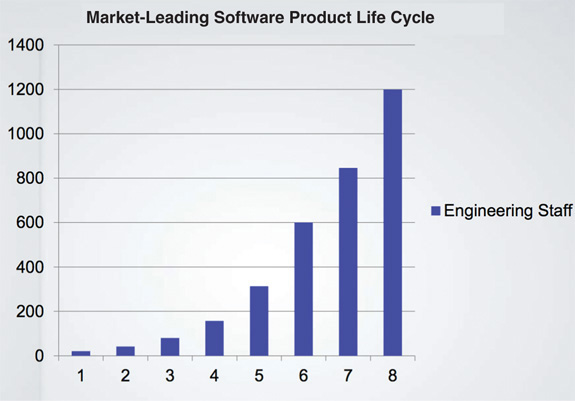
\includegraphics[width=0.8\linewidth]{images/EA/diagram_growth_of_staff.jpg}
    \caption{Personalzuwachs \\ \cite[S. 5]{EA:Book01}}
    \label{fig:personnel-growth}
\end{figure}

In der Abbildung \ref{fig:personnel-growth} wird dargestellt, wie der Personalaufwand im Laufe der Zeit ansteigt.
Das Balkendiagramm zeigt dabei, wie viele Ingenieur/innen an einem bestimmten Release beteiligt sind.

Ein Personalzuwachs muss grundsätzlich nicht negativ sein. Allerdings kann eine zunehmend komplexe und schwer veränderbare Architektur dazu führen, dass immer mehr Personal benötigt wird, um die Software zu warten und weiterzuentwickeln. 
Eine solche Entwicklung geht häufig mit einer sinkenden Produktivität des Teams einher, da die steigende Komplexität die Effizienz beeinträchtigt und die Implementierung neuer Funktionen erschwert.

\clearpage

\begin{figure}[H]
    \centering
    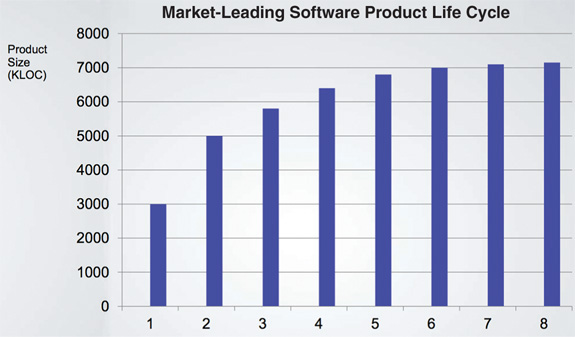
\includegraphics[width=0.8\linewidth]{images/EA/diagram_productivity.jpg}
    \caption{Produktivität \\ \cite[S. 6]{EA:Book01}}
    \label{fig:productivity}
\end{figure}

Betrachtet man anschließend die Abbildung \ref{fig:productivity}, wird die oben genannte Problematik deutlich.
Die Produktivität wird hier anhand der geschriebenen Codezeilen gemessen, was zwar wenig darüber aussagt, ob tatsächlich neue Funktionen oder Änderungen erfolgreich umgesetzt wurden. Mehr Code bedeutet schließlich nicht zwangsläufig, dass dadurch bessere Ergebnisse erzielt werden.

Zu Beginn scheint die Produktivität zwar zu steigen, nähert sich jedoch ab einem gewissen Punkt einer Asymptote\footnote{Linie, der sich eine Kurve immer weiter annähert, ohne sie jemals zu berühren}. Das bedeutet, dass das Hinzufügen weiterer Ressourcen nicht automatisch zu einer Steigerung der Produktivität führt. 

Das Problem dabei ist nicht nur, dass das Unternehmen weitere Personen einstellen und bezahlen muss, sondern auch, dass die derzeitigen Mitarbeiter/innen darunter leiden könnten. Eine abnehmende Produktivität kann zu \textbf{Motivationsverlust} führen, sodass Mitarbeitende im schlimmsten Fall sogar das Unternehmen verlassen. 
\cite[S. 5-10]{EA:Book01} 

\begin{figure}[H]
    \centering
    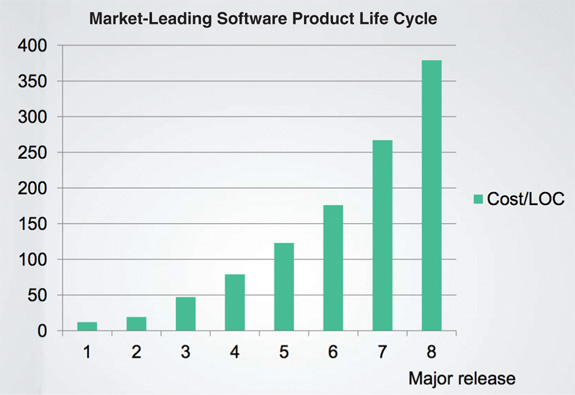
\includegraphics[width=0.7\linewidth]{images/EA/diagram_costs.jpg}
    \caption{Kostenentwicklung \\ \cite[S. 7]{EA:Book01}}
    \label{fig:cost-development}
\end{figure}

Ein Blick auf die Entwicklung der Kosten in Abbildung \ref{fig:cost-development} zeigt, dass die Kosten trotz kaum ansteigender Produktivität (siehe Abbildung \ref{fig:productivity}) und steigendem Personalbedarf (siehe Abbildung \ref{fig:personnel-growth}) immer weiter steigen. Dies bedeutet, dass der \textbf{Kunde oder die Kundin enorme Summen für kaum sichtbare Fortschritte investiert}. 

Ist der Kunde oder die Kundin nicht gewillt, dafür zu bezahlen, kann dies zum Abbruch des Projekts führen, wodurch das Unternehmen in ein schlechtes Licht gerückt wird und im schlimmsten Fall mit der Auflösung des Unternehmens enden kann. \\
\cite[S. 5-10]{EA:Book01} 

% --- Ü B E R L E I T U N G   Z U R   A N F O R D E R U N G S A N A L Y S E ---

All diese Probleme können durch eine \glqq gute\grqq\ Softwarearchitektur vermieden werden. Doch was versteht man darunter? Was ist gut und was ist schlecht? Fakt ist, dass es keine universelle Lösung für die Softwarearchitektur gibt. Abhängig vom Anwendungsfall, Anforderungen, Teamgröße und vielen weiteren Faktoren kann eine andere Architektur vorteilhaft sein.
Im weiteren Verlauf wird näher auf die Anforderungen einer Software eingegangen, die notwendig sind, um einen passenden Architekturstil auszuwählen.
